\documentclass[letterpaper,journal]{IEEEtran}
\usepackage{cite}
\usepackage{amsmath,amsfonts,amssymb}
\usepackage{array}
\usepackage[caption=false,font=normalsize,labelfont=sf,textfont=sf]{subfig}
\usepackage{textcomp}
\usepackage{stfloats}
\usepackage{url}
\usepackage{graphicx}
\usepackage{balance}
\hyphenation{Koop-man pre-dic-tive}
\def\BibTeX{{\rm B\kern-.05em{\sc i\kern-.025em b}\kern-.08em
    T\kern-.1667em\lower.7ex\hbox{E}\kern-.125emX}}

\newtheorem{assumption}{Assumption}
\newtheorem{proposition}{Proposition}
\newtheorem{remark}{Remark}

\begin{document}

\title{Tube-Tightened Bilinear Koopman Model Predictive Guidance With Impact-Time and Impact-Angle Constraints}

\author{Qiuya Li
\thanks{This manuscript is a working draft prepared from the current Koopman guidance workspace. The author affiliation and funding information should be completed before submission.}}

\markboth{Working Draft, Koopman Guidance Manuscript, 2026}%
{Li: Tube-Tightened Bilinear Koopman Model Predictive Guidance}

\maketitle

\begin{abstract}
This paper investigates a Koopman-operator-based model predictive guidance method for a planar stationary-target engagement subject to simultaneous impact-time and impact-angle constraints. The finite-time interception condition is difficult to handle in the original relative-motion coordinates because the target point is not an equilibrium of the constant-speed pursuer dynamics. To address this issue, a time-to-go lateral-error model is constructed, in which the prescribed impact time, cross-track displacement, and terminal heading error are represented by a terminal origin. It is first shown that the ideal Cartesian acceleration-controlled model admits an exact finite-dimensional continuous-time bilinear Koopman representation under the constant-speed stationary-target assumption. Based on this structure, a bilinear extended dynamic mode decomposition predictor is learned and embedded into a sequential convex Koopman model predictive control scheme. The implemented predictor further includes a first-order autopilot state, so that the optimized command is filtered before acting on the flight-path dynamics. A validation-data residual tube is introduced to tighten the terminal constraints and to connect nominal predicted feasibility with the original impact constraints. Numerical simulations with a 10 m capture radius show that the proposed method satisfies the prescribed impact time of 21.7 s and impact angle of $-2^\circ$, achieving a 5.978 m terminal miss distance and a $0.647^\circ$ impact-angle error without quadratic-program failures. Additional nominal scenarios indicate that the same controller structure also satisfies a slightly delayed 21.75 s terminal-time command, while earlier, later, or substantially different impact-angle commands can leave the 10 m capture set. These results demonstrate that the time-to-go bilinear Koopman formulation provides a tractable predictive-guidance framework for nominal multi-constraint interception and a useful diagnostic tool for terminal reachability.
\end{abstract}

\begin{IEEEkeywords}
Koopman operator, model predictive guidance, impact-angle constraint, impact-time constraint, residual tube, bilinear predictor.
\end{IEEEkeywords}

\section{Introduction}
\IEEEPARstart{T}{erminal} guidance with multiple impact constraints is a central problem in precision engagement. In addition to reducing miss distance, a guidance law may be required to satisfy a prescribed impact angle and a specified impact time. These two terminal constraints are coupled through the remaining trajectory: an impact-angle command shapes the terminal direction of motion, while an impact-time command determines how quickly the pursuer must spend its remaining range. As a result, the guidance command must regulate the whole terminal engagement rather than only reduce the instantaneous line-of-sight rate.

Model predictive control (MPC) is attractive for this setting because terminal and path constraints can be imposed explicitly. Its direct nonlinear implementation, however, may be computationally burdensome in real-time guidance. Koopman operator methods provide an alternative route: nonlinear dynamics are represented in a lifted observable space in which prediction can be approximately linear or structured bilinear. This idea has been used in Koopman-based MPC and recently in Koopman-operator-based integrated guidance and control for strap-down high-speed missiles, where a Koopman predictor is combined with Lyapunov-based MPC to handle nonlinearities and constraints \cite{zhou2024klmpc}. Following this predictor-then-MPC design logic, this paper focuses on impact-time and impact-angle constrained guidance for a stationary target and addresses a specific theoretical issue: the terminal intercept condition is not an equilibrium in the original relative-motion coordinates.

The main contributions are summarized as follows.
\begin{enumerate}
    \item A finite-dimensional continuous-time bilinear Koopman representation is derived for the constant-speed stationary-target guidance model in Cartesian relative coordinates. This result clarifies why a bilinear lifted predictor is more consistent with the control-affine guidance dynamics than a purely linear input predictor.
    \item A time-to-go lateral-error state $x_\tau=[\tau/t_f,\;y/R_s,\;\theta]^T$ is introduced to convert the impact-time, cross-track, and impact-angle requirements into a terminal-origin condition suitable for predictive guidance.
    \item A sequential convex bilinear Koopman-MPC law is constructed with interpolation between measured and predicted lifted states, an input-difference penalty, terminal slack variables, and residual-tube terminal tightening.
    \item Nominal simulations verify the prediction accuracy and constrained terminal performance of the proposed method under a 10 m capture-radius requirement.
\end{enumerate}

The remainder of this paper is organized as follows. Section II formulates the engagement model and terminal constraints. Section III derives the exact continuous-time bilinear Koopman representation. Section IV constructs the time-to-go terminal-error model. Section V presents the bilinear EDMD predictor and the sequential convex Koopman-MPC design. Section VI develops the residual-tube terminal tightening. Section VII reports nominal simulation results, and Section VIII concludes the paper.

\section{Planar Guidance Problem}

\subsection{Relative Motion}
Consider a stationary target at the origin and a pursuer moving at constant nominal speed $V>0$ in the planar engagement. Let
\begin{equation}
    r=\begin{bmatrix}r_x&r_y\end{bmatrix}^T,\qquad
    \gamma\in\mathbb R
\end{equation}
denote the relative position and flight-path angle, respectively. The ideal lateral acceleration command is $A$, and the normalized command is
\begin{equation}
    u=\frac{A}{A_{\max}},\qquad |u|\le 1 .
\end{equation}
The ideal acceleration-controlled guidance core is
\begin{equation}
    \dot r_x=-V\cos\gamma,\qquad
    \dot r_y=-V\sin\gamma,\qquad
    \dot\gamma=\frac{A_{\max}}{V}u .
    \label{eq:cartesian_model}
\end{equation}
The closed-loop simulations additionally pass the optimized command $u_c$ through a first-order autopilot,
\begin{equation}
    \dot\gamma=\frac{A_{\max}}{V}u_a,\qquad
    \tau_a\dot u_a=-u_a+u_c,\qquad |u_c|\le1 ,
    \label{eq:autopilot}
\end{equation}
where $u_a$ is the actual normalized lateral acceleration. The ideal model \eqref{eq:cartesian_model} is recovered when $u_a=u_c=u$. The simulations use $V=300$ m/s, $A_{\max}=100$ m/s$^2$, sampling period $T_s=0.1$ s, and autopilot time constant $\tau_a=0.10$ s.

\begin{assumption}
The target is stationary, the pursuer speed is constant within each case, the command $u$ is piecewise constant and bounded, and the engagement is considered before the singular intercept instant. The heading angle is treated as an unwrapped real variable when differentiability is needed.
\end{assumption}

\subsection{Impact-Time and Impact-Angle Constraints}
Let $t_f$ be the prescribed impact time and $\gamma_f$ be the prescribed impact angle. The terminal requirements are
\begin{equation}
    \|r(t_f)\|\le r_c,\qquad
    |\gamma(t_f)-\gamma_f|\le \varepsilon_\gamma ,
    \label{eq:terminal_requirements}
\end{equation}
where the current implementation uses $r_c=10$ m and $\varepsilon_\gamma=3^\circ$. The scheduled-time tolerance is one half sampling period, i.e., $\varepsilon_t=T_s/2$.

The main conceptual difficulty is that $r=0$ is not an equilibrium of \eqref{eq:cartesian_model}. Even if the pursuer reaches the target, $\dot r$ remains nonzero. Thus, terminal stability and recursive-feasibility arguments cannot be copied directly from regulation MPC in the original Cartesian state. A terminal coordinate must encode the remaining time-to-go and lateral impact error.

\section{Koopman Modeling Structure}

\subsection{Controlled Koopman Generator}
For a controlled nonlinear system
\begin{equation}
    \dot x=f_0(x)+u f_1(x),
\end{equation}
the controlled Koopman generator acting on a smooth observable $g$ is
\begin{equation}
    \mathcal L_u g(x)=\nabla g(x)^T(f_0(x)+u f_1(x))
    =\mathcal L_0g(x)+u\mathcal L_1g(x).
\end{equation}
This formulation should be interpreted as a representation of the controlled generator, not as a single autonomous Koopman operator independent of the input.

\subsection{Why Polar Observables Do Not Close Finitely}
In polar line-of-sight coordinates with range $R$, line-of-sight angle $\lambda$, and heading error $\sigma=\gamma-\lambda$, the usual kinematics are
\begin{equation}
    \dot R=-V\cos\sigma,\quad
    \dot\lambda=-\frac{V\sin\sigma}{R},\quad
    \dot\gamma=\frac{A_{\max}}{V}u .
\end{equation}
If the observable dictionary contains $1/R$, $\sin\sigma$, and $\cos\sigma$, then repeated differentiation generates terms such as $R^{-2}$, $\sin\sigma\cos\sigma/R$, and higher rational-trigonometric products. Hence a small finite dictionary of conventional polar observables does not generally yield exact linear-in-input closure. EDMD can still approximate the dynamics on a bounded operating domain, but the residual must be explicitly treated.

\subsection{Exact Continuous-Time Bilinear Lift}
In Cartesian relative coordinates, the situation is different. Define the lifted state
\begin{equation}
    z=
    \begin{bmatrix}
    1&r_x&r_y&\gamma&\cos\gamma&\sin\gamma
    \end{bmatrix}^T .
    \label{eq:exact_lift}
\end{equation}
Then the observable span generated by \eqref{eq:exact_lift} is invariant under $\mathcal L_0$ and $\mathcal L_1$. Specifically,
\begin{equation}
    \mathcal L_0 r_x=-V\cos\gamma,\qquad
    \mathcal L_0 r_y=-V\sin\gamma ,
\end{equation}
\begin{equation}
\begin{aligned}
    \mathcal L_1 \gamma&=\frac{A_{\max}}{V},\\
    \mathcal L_1 \cos\gamma&=-\frac{A_{\max}}{V}\sin\gamma,\\
    \mathcal L_1 \sin\gamma&=\frac{A_{\max}}{V}\cos\gamma .
\end{aligned}
\end{equation}
Therefore
\begin{equation}
    \dot z=A_0z+uB_1z ,
    \label{eq:exact_bilinear}
\end{equation}
where the nonzero entries are
\begin{equation}
    A_0(2,5)=-V,\quad A_0(3,6)=-V,
\end{equation}
\begin{equation}
\begin{aligned}
    B_1(4,1)&=\frac{A_{\max}}{V},\\
    B_1(5,6)&=-\frac{A_{\max}}{V},\\
    B_1(6,5)&=\frac{A_{\max}}{V}.
\end{aligned}
\end{equation}

\begin{proposition}
Under Assumption 1, the planar stationary-target guidance model \eqref{eq:cartesian_model} admits the exact finite-dimensional continuous-time bilinear Koopman representation \eqref{eq:exact_bilinear} on the observable space spanned by \eqref{eq:exact_lift}.
\end{proposition}

\begin{remark}
The exact continuous-time bilinear representation is not the same object as the finite-dimensional predictor used inside the online quadratic program. Under zero-order-hold input, the exact discrete lifted map is $z_{k+1}=\exp(T_s(A_0+u_kB_1))z_k$, which depends nonlinearly on $u_k$. The data-driven predictor below is therefore a tractable approximation on a prescribed operating domain.
\end{remark}

\section{Time-to-Go Lateral-Error State}

Let
\begin{equation}
    e_f=\begin{bmatrix}\cos\gamma_f\\ \sin\gamma_f\end{bmatrix},\qquad
    n_f=\begin{bmatrix}-\sin\gamma_f\\ \cos\gamma_f\end{bmatrix}.
\end{equation}
Define the along-impact distance, cross-track displacement, and heading error as
\begin{equation}
    s=e_f^Tr,\qquad y=n_f^Tr,\qquad \theta=\gamma-\gamma_f .
\end{equation}
The geometric time-to-go coordinate is
\begin{equation}
    \tau=\frac{s}{V}.
\end{equation}
Then
\begin{equation}
    r=V\tau e_f+yn_f,\qquad
    \|r\|^2=V^2\tau^2+y^2 .
    \label{eq:r_tau_y}
\end{equation}
The terminal intercept condition $r=0$ and $\gamma=\gamma_f$ is therefore equivalent to
\begin{equation}
    \tau=0,\qquad y=0,\qquad \theta=0 .
    \label{eq:terminal_origin}
\end{equation}
This is the key reason for using the time-to-go lateral-error state. In normalized form, the prediction output is chosen as
\begin{equation}
    x_\tau=
    \begin{bmatrix}
    \tau/t_f&y/R_s&\theta
    \end{bmatrix}^T,
    \label{eq:xtau}
\end{equation}
where $R_s=6000$ m in the simulations.

The nominal dynamics in $(\tau,y,\theta)$ are
\begin{equation}
    \dot\tau=-\cos\theta,\qquad
    \dot y=-V\sin\theta,\qquad
    \dot\theta=\frac{A_{\max}}{V}u .
    \label{eq:tgo_dynamics}
\end{equation}
With the first-order autopilot, $u$ in \eqref{eq:tgo_dynamics} is replaced by $u_a$ and the additional actuator state obeys \eqref{eq:autopilot}. The terminal origin remains $(\tau,y,\theta)=(0,0,0)$; the actuator state is not itself a terminal impact constraint.
Near $\theta=0$, the lateral subsystem is
\begin{equation}
    \dot y=-V\theta+O(\theta^3),\qquad
    \dot\theta=\frac{A_{\max}}{V}u .
\end{equation}
A local terminal controller can therefore be selected as
\begin{equation}
    u=\kappa(y,\theta)=k_y y-k_\theta\theta ,
\end{equation}
with gains chosen so that the local linearization is stable and the command remains within the available acceleration limit. Let $P_f\succ0$ solve the Lyapunov equation
\begin{equation}
    A_c^TP_f+P_fA_c=-Q_f,\qquad Q_f\succ0 ,
\end{equation}
where $A_c$ is the local closed-loop lateral-error matrix. A Lyapunov terminal set can be written as
\begin{equation}
    \mathcal X_f(\tau)=
    \{(y,\theta):[y,\theta]P_f[y,\theta]^T\le\alpha,
    |\kappa(y,\theta)|\le 1-\eta_u\}.
    \label{eq:terminal_set}
\end{equation}
The current implementation uses a polyhedral approximation of the terminal tolerances in \eqref{eq:terminal_origin}, tightened by the residual tube. Equation \eqref{eq:terminal_set} gives the rigorous terminal-set direction for the next theoretical refinement.

\section{Bilinear EDMD Predictor and Sequential Convex MPC}

\subsection{Lifted Dictionary and Identification}
The implemented lifted dictionary for the normalized time-to-go state and first-order autopilot state is
\begin{align}
    \psi(x_\tau,u_a)=
    [&1,\tau,y,\theta,u_a,\cos\theta,\sin\theta,
    \tau\cos\theta,\tau\sin\theta, \nonumber\\
    &y\cos\theta,y\sin\theta,\theta^2,
    u_a\cos\theta,u_a\sin\theta]^T .
    \label{eq:dictionary}
\end{align}
Here $\tau$ and $y$ denote the normalized components in \eqref{eq:xtau}. The output matrix extracts $[\tau/t_f,y/R_s,\theta]^T$ from the lifted state, while $u_a$ is retained to represent actuator lag. From sampled data, the bilinear EDMD predictor is identified as
\begin{equation}
    z_{k+1}=A_b z_k+B_0u_k+u_kB_bz_k+w_k ,
    \label{eq:bilinear_predictor}
\end{equation}
where $z_k=\psi(x_{\tau,k})$ and $w_k$ is the finite-dimensional prediction residual. The regression matrix is
\begin{equation}
    \Omega_b=
    \begin{bmatrix}
    Z_-\\ U_-\\ U_-\odot Z_-
    \end{bmatrix},
\end{equation}
and the ridge-regression estimate is
\begin{equation}
    [A_b\;B_0\;B_b]=Z_+\Omega_b^T
    (\Omega_b\Omega_b^T+\rho I)^{-1}.
\end{equation}

\subsection{Sequential Convex Approximation}
Direct MPC with \eqref{eq:bilinear_predictor} is nonconvex because of the product $u_kB_bz_k$. At each sampling instant, the controller uses a small number of sequential convex iterations. Given a nominal lifted trajectory $\bar z_{i|k}$, define
\begin{equation}
    B_{{\rm eff},i}=B_0+B_b\bar z_{i|k}.
\end{equation}
The local prediction model is then
\begin{equation}
    z_{i+1|k}=A_bz_{i|k}+B_{{\rm eff},i}u_{i|k}.
    \label{eq:ltv_prediction}
\end{equation}
The optimized control sequence is damped between iterations to avoid numerical chattering caused by the bilinear approximation.

\subsection{Interpolated Initial Lifted State}
Let $z_k^m$ be the measured lifted state and $z_k^p$ be the previously predicted current lifted state. The initial lifted state for the current horizon is interpolated as
\begin{equation}
    z_{0|k}=z_k^m+\xi_k(z_k^p-z_k^m),\qquad 0\le \xi_k\le 1 .
    \label{eq:interpolation}
\end{equation}
This follows the stabilizing idea of interpolating between measured and predicted lifted states used in Koopman data-driven predictive control \cite{dejong2024kdpc}. The interpolation variable is penalized so that the controller uses it only when prediction mismatch would otherwise degrade feasibility.

\subsection{Quadratic Program}
Let $\mathbf U_k=[u_{0|k},\ldots,u_{N-1|k}]^T$ and let the stacked predicted outputs be affine in the decision variables after linearization:
\begin{equation}
    \mathbf X_k=c_k+M_k
    \begin{bmatrix}
    \mathbf U_k\\ \xi_k
    \end{bmatrix}.
\end{equation}
The online optimization is
\begin{align}
    \min_{\mathbf U_k,\xi_k,s_f}\quad
    &\|\mathbf X_k-\mathbf X_k^{\rm ref}\|_{\bar Q}^2
    +\|\mathbf U_k\|_{\bar R}^2
    +\|D\mathbf U_k-d_{u,k}\|_{R_\Delta}^2 \nonumber\\
    &+\|z_k^m+\xi_k(z_k^p-z_k^m)\|_{Q_0}^2 \nonumber\\
    &+\lambda \xi_k^2\|z_k^p-z_k^m\|^2
    +\|s_f\|_{S_f}^2
    \label{eq:qp_cost}
\end{align}
subject to
\begin{equation}
    -1\le u_{i|k}\le 1,\qquad 0\le \xi_k\le 1,\qquad s_f\ge0,
\end{equation}
the heading path constraint
\begin{equation}
    |\gamma_f+\theta_{i|k}|\le \gamma_{\max},
\end{equation}
and terminal constraints on the scheduled terminal prediction step. The matrix $D$ is the first-difference matrix, so that the term with $R_\Delta$ penalizes $u_{0|k}-u_{k-1}$ and $u_{i|k}-u_{i-1|k}$. This term suppresses acceleration chattering.

For the impact-time-and-angle mode, the terminal target is
\begin{equation}
    \left|
    \begin{bmatrix}
    \tau_{N|k}/t_f\\ y_{N|k}/R_s\\ \theta_{N|k}
    \end{bmatrix}
    -
    \begin{bmatrix}
    0\\0\\0
    \end{bmatrix}
    \right|
    \le \varepsilon^{\rm tight}+s_f .
\end{equation}
\section{Residual Tube Tightening}

\subsection{Multi-Step Residual Tube}
Let $X_{h,j}^{\rm true}$ and $X_{h,j}^{\rm pred}$ denote the true and predicted $x_\tau$ outputs at prediction step $h$ for validation case $j$. The componentwise residual tube is estimated by
\begin{equation}
    \rho_h=\alpha_\rho\operatorname{quantile}_{0.99}
    \{|X_{h,j}^{\rm true}-X_{h,j}^{\rm pred}|\}_j ,
    \label{eq:tube_bound}
\end{equation}
where $\alpha_\rho=1.2$ is an inflation factor. The tightened terminal tolerance at step $h$ is
\begin{equation}
    \varepsilon_h^{\rm tight}=
    \varepsilon-\min\{\eta_{\max}\varepsilon,\rho_h\},
    \label{eq:tightening}
\end{equation}
with $\eta_{\max}=0.8$. In the default simulation, the terminal 99\% tube bound for $[\tau/t_f,y/R_s,\theta]^T$ is
\begin{equation}
    [7.199{\times}10^{-5},\;8.467{\times}10^{-5},\;4.036{\times}10^{-7}]^T .
\end{equation}
For $r_c=10$ m, the nominal terminal tolerance is
\begin{equation}
    [1.536{\times}10^{-3},\;1.667{\times}10^{-3},\;5.236{\times}10^{-2}]^T,
\end{equation}
and the tightened tolerance is
\begin{equation}
    [1.464{\times}10^{-3},\;1.582{\times}10^{-3},\;5.236{\times}10^{-2}]^T .
\end{equation}

\subsection{ISS Interpretation}
Let $\chi=[y,\theta]^T$ denote the lateral terminal error and suppose the true error dynamics under a local terminal feedback satisfy
\begin{equation}
    \chi_{k+1}=F_\chi(\chi_k,u_k,\tau_k)+d_k,\qquad d_k\in\mathcal D .
\end{equation}
If there exists a terminal Lyapunov function $V_f$ such that
\begin{equation}
    V_f(F_\chi(\chi,\kappa(\chi),\tau)+d)-V_f(\chi)
    \le -\ell_f(\chi)+c_d\|d\|^2 ,
    \label{eq:iss_condition}
\end{equation}
then the terminal closed loop is input-to-state stable with respect to the prediction disturbance. The residual tube in \eqref{eq:tube_bound} and the tightening in \eqref{eq:tightening} are the numerical mechanism used here to connect nominal predicted feasibility with true constraint satisfaction.

\section{Numerical Results}

\subsection{Simulation Setup}
The stationary-target engagement starts from
\begin{equation}
    r(0)=
    \begin{bmatrix}
    6000&1500
    \end{bmatrix}^T{\rm m},\qquad
    \gamma(0)=25^\circ .
\end{equation}
The nominal speed is $300$ m/s, $T_s=0.1$ s, $R_s=6000$ m, $A_{\max}=100$ m/s$^2$, $\tau_a=0.10$ s, and the prediction horizon is $N=35$. The prescribed default terminal conditions are $t_f=21.7$ s and $\gamma_f=-2^\circ$. The data set contains 260 training trajectories and 60 test trajectories for the default run. All online optimizations are solved as convex quadratic programs after sequential convexification.

\subsection{Prediction Accuracy}
The exact bilinear lift of the ideal acceleration-controlled core was checked by integrating the lifted and original systems with the same Runge-Kutta scheme for 300 steps. The maximum consistency error was $3.99\times10^{-11}$, confirming the exact continuous-time closure of the core model. The autopilot-augmented predictor is then evaluated through validation-data prediction errors and residual-tube tightening.

Table \ref{tab:prediction} compares one-step linear EDMD, direct 35-step linear EDMD, and the bilinear rolling predictor used by the controller. The bilinear rolling predictor substantially reduces long-horizon normalized errors in the time-to-go and cross-track components compared with the direct linear multi-step predictor.

\begin{table}[!t]
\caption{Prediction Error on the Test Set}
\label{tab:prediction}
\centering
\begin{tabular}{c c c c}
\hline
State & One-step & Linear 35-step & Bilinear rolling\\
\hline
$\tau/t_f$ & $6.94{\times}10^{-6}$ & $2.28{\times}10^{-2}$ & $3.92{\times}10^{-5}$\\
$y/R_s$ & $3.04{\times}10^{-6}$ & $9.87{\times}10^{-3}$ & $3.29{\times}10^{-5}$\\
$\theta$ & $2.35{\times}10^{-9}$ & $9.64{\times}10^{-9}$ & $7.09{\times}10^{-8}$\\
\hline
\end{tabular}
\end{table}

\begin{figure}[!t]
\centering
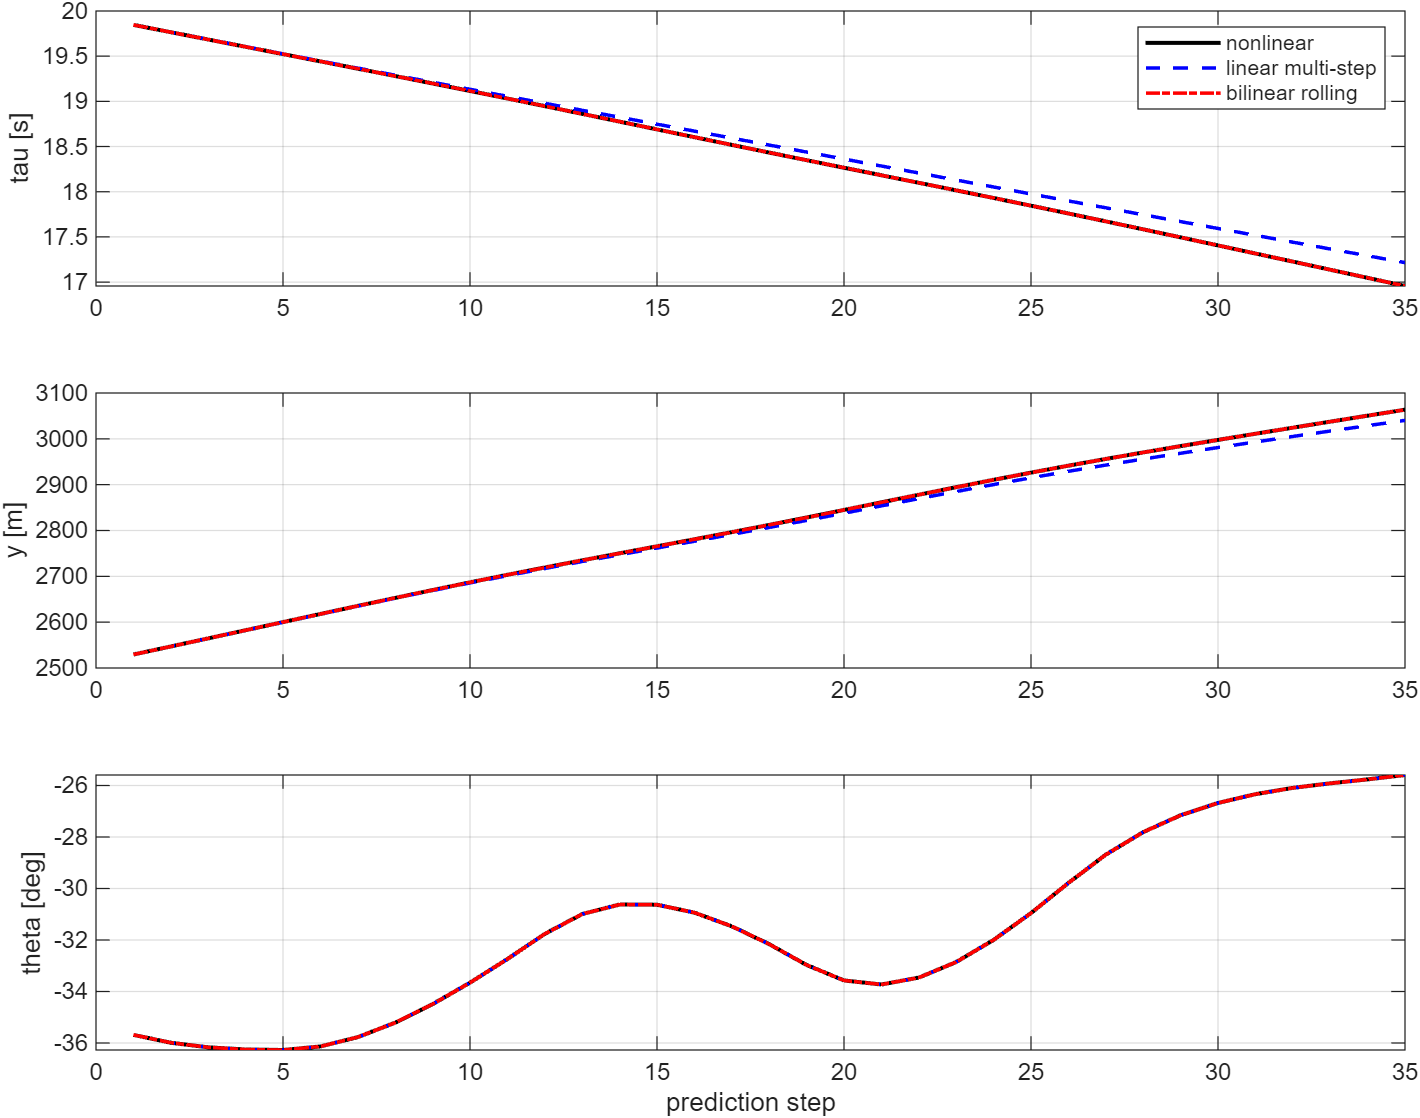
\includegraphics[width=3.35in]{KDPC_RSRFG-main/StationaryTargetKoopman/results/prediction_validation.png}
\caption{Prediction comparison between the nonlinear trajectory, the direct linear multi-step EDMD predictor, and the rolling bilinear Koopman predictor.}
\label{fig:prediction}
\end{figure}

\subsection{Impact-Time and Impact-Angle Guidance}
The nominal constrained case uses a 10 m capture radius, $t_f=21.7$ s, and $\gamma_f=-2^\circ$. Table \ref{tab:default} reports the closed-loop terminal performance. The proposed guidance law satisfies the scheduled impact-time constraint with zero sampling-level time error. At the scheduled impact instant, the terminal miss distance is 5.978 m, which is inside the prescribed 10 m capture radius, and the impact-angle error is $0.647^\circ$, which is inside the $3^\circ$ tolerance. No quadratic-program failure occurs during the closed-loop simulation.

\begin{table}[!t]
\caption{Default Impact-Time and Impact-Angle Case}
\label{tab:default}
\centering
\begin{tabular}{c c c c c}
\hline
Case & Satisfied & Time error & Miss & Angle error\\
\hline
Nominal & Yes & 0.00 s & 5.978 m & $0.647^\circ$\\
\hline
\end{tabular}
\end{table}

\begin{figure}[!t]
\centering
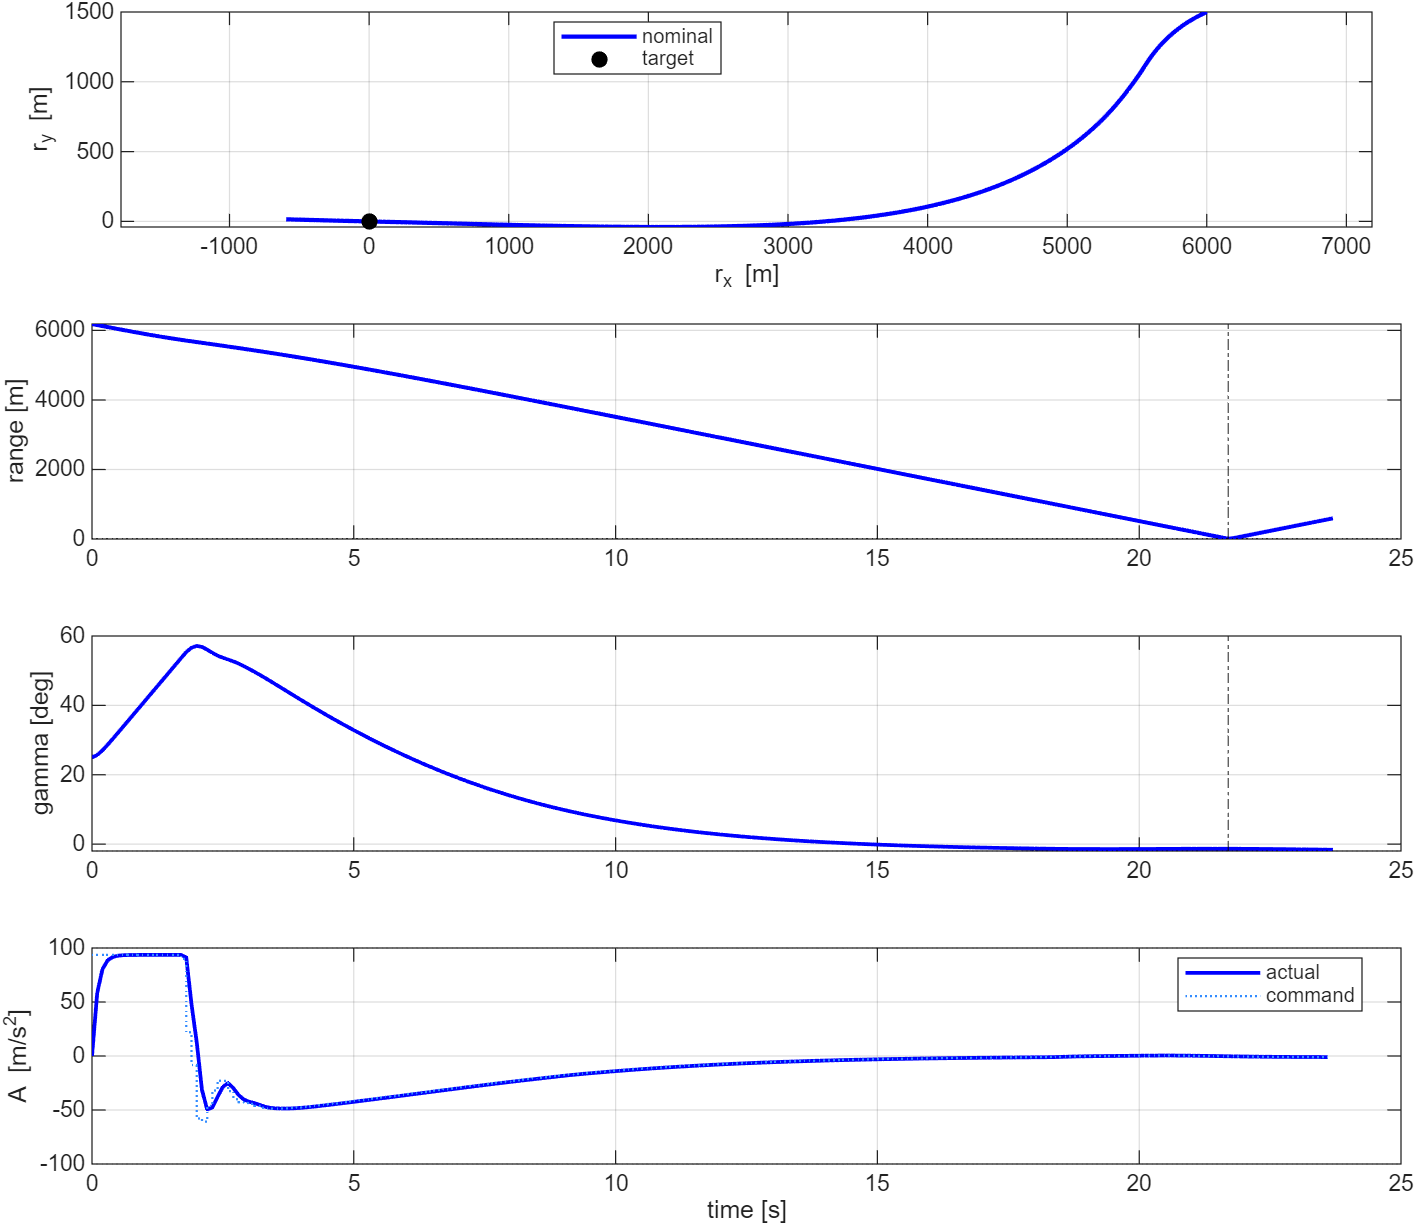
\includegraphics[width=3.35in]{KDPC_RSRFG-main/StationaryTargetKoopman/results/closed_loop_nominal.png}
\caption{Nominal closed-loop trajectory, range history, heading response, and lateral acceleration for the impact-time and impact-angle constrained case. The solid acceleration curve is the first-order-autopilot output, while the dotted curve is the MPC command.}
\label{fig:closed_loop}
\end{figure}

Fig. \ref{fig:closed_loop} shows the closed-loop response. The range decreases to the capture neighborhood at the prescribed terminal time, while the heading converges to the desired impact angle. The commanded and actual accelerations remain within the 100 m/s$^2$ limit. The input-difference penalty suppresses command chattering, and the first-order autopilot makes the applied acceleration continuous.

\subsection{Additional Nominal Scenario Tests}
To further examine the terminal-constraint envelope, additional nominal cases were tested by changing either the prescribed impact time or the prescribed impact angle. Table \ref{tab:full_cases} gives two full-data successful cases. Besides the baseline 21.70 s command, the controller also satisfies a slightly delayed 21.75 s command with a 9.794 m miss distance and a $0.530^\circ$ angle error. Both cases satisfy the 10 m capture-radius requirement and have no quadratic-program failures.

\begin{table}[!t]
\caption{Full-Data Successful Nominal Cases}
\label{tab:full_cases}
\centering
\begin{tabular}{c c c c c}
\hline
$t_f$ [s] & $\gamma_f$ [deg] & Satisfied & Miss [m] & Angle error [deg]\\
\hline
21.70 & -2 & Yes & 5.978 & 0.647\\
21.75 & -2 & Yes & 9.794 & 0.530\\
\hline
\end{tabular}
\end{table}

Table \ref{tab:screening_cases} reports a nominal screening study with reduced identification data. The results show that the feasible time window is narrow under the current 10 m capture radius, 3.5 s prediction horizon, and acceleration bound. When $\gamma_f=-2^\circ$, the 21.70 s and 21.75 s cases enter the capture set, whereas the 21.60 s and 21.80 s cases miss the 10 m terminal set. At the fixed impact time of 21.70 s, changing the prescribed angle to $-8^\circ$, $0^\circ$, or $5^\circ$ also violates the capture-radius requirement. These cases do not indicate quadratic-program failure; instead, they expose the reachable terminal envelope of the present nominal design.

\begin{table}[!t]
\caption{Nominal Screening Cases for Terminal Reachability}
\label{tab:screening_cases}
\centering
\begin{tabular}{c c c c}
\hline
$t_f$ [s] & $\gamma_f$ [deg] & Miss [m] & Angle error [deg]\\
\hline
21.60 & -2 & 28.617 & 0.869\\
21.70 & -2 & 5.915 & 0.468\\
21.75 & -2 & 9.613 & 0.415\\
21.80 & -2 & 16.575 & 0.362\\
21.70 & -8 & 143.809 & 1.393\\
21.70 & 0 & 43.696 & 0.028\\
21.70 & 5 & 157.849 & -0.074\\
\hline
\end{tabular}
\end{table}

The impact-angle-only cases requested in the preliminary study were also included as nominal flight simulations. In these tests, the terminal time is not prescribed; the controller enforces the terminal angle and cross-track capture condition while using the time-to-go component only as a progress reference. Table \ref{tab:angle_only_nominal} reports the 30$^\circ$ and 45$^\circ$ results. Both cases satisfy the 10 m capture-radius condition and the 3$^\circ$ impact-angle tolerance. The corresponding flight responses are shown in Fig. \ref{fig:angle_only_nominal}.

\begin{table}[!t]
\caption{Nominal Impact-Angle-Only Cases}
\label{tab:angle_only_nominal}
\centering
\begin{tabular}{c c c c c}
\hline
$\gamma_f$ [deg] & Time [s] & Satisfied & Miss [m] & Angle error [deg]\\
\hline
30 & 22.10 & Yes & 6.945 & -0.107\\
45 & 22.90 & Yes & 7.280 & -0.404\\
\hline
\end{tabular}
\end{table}

\begin{figure*}[!t]
\centering
\subfloat[30$^\circ$ impact-angle command.]{
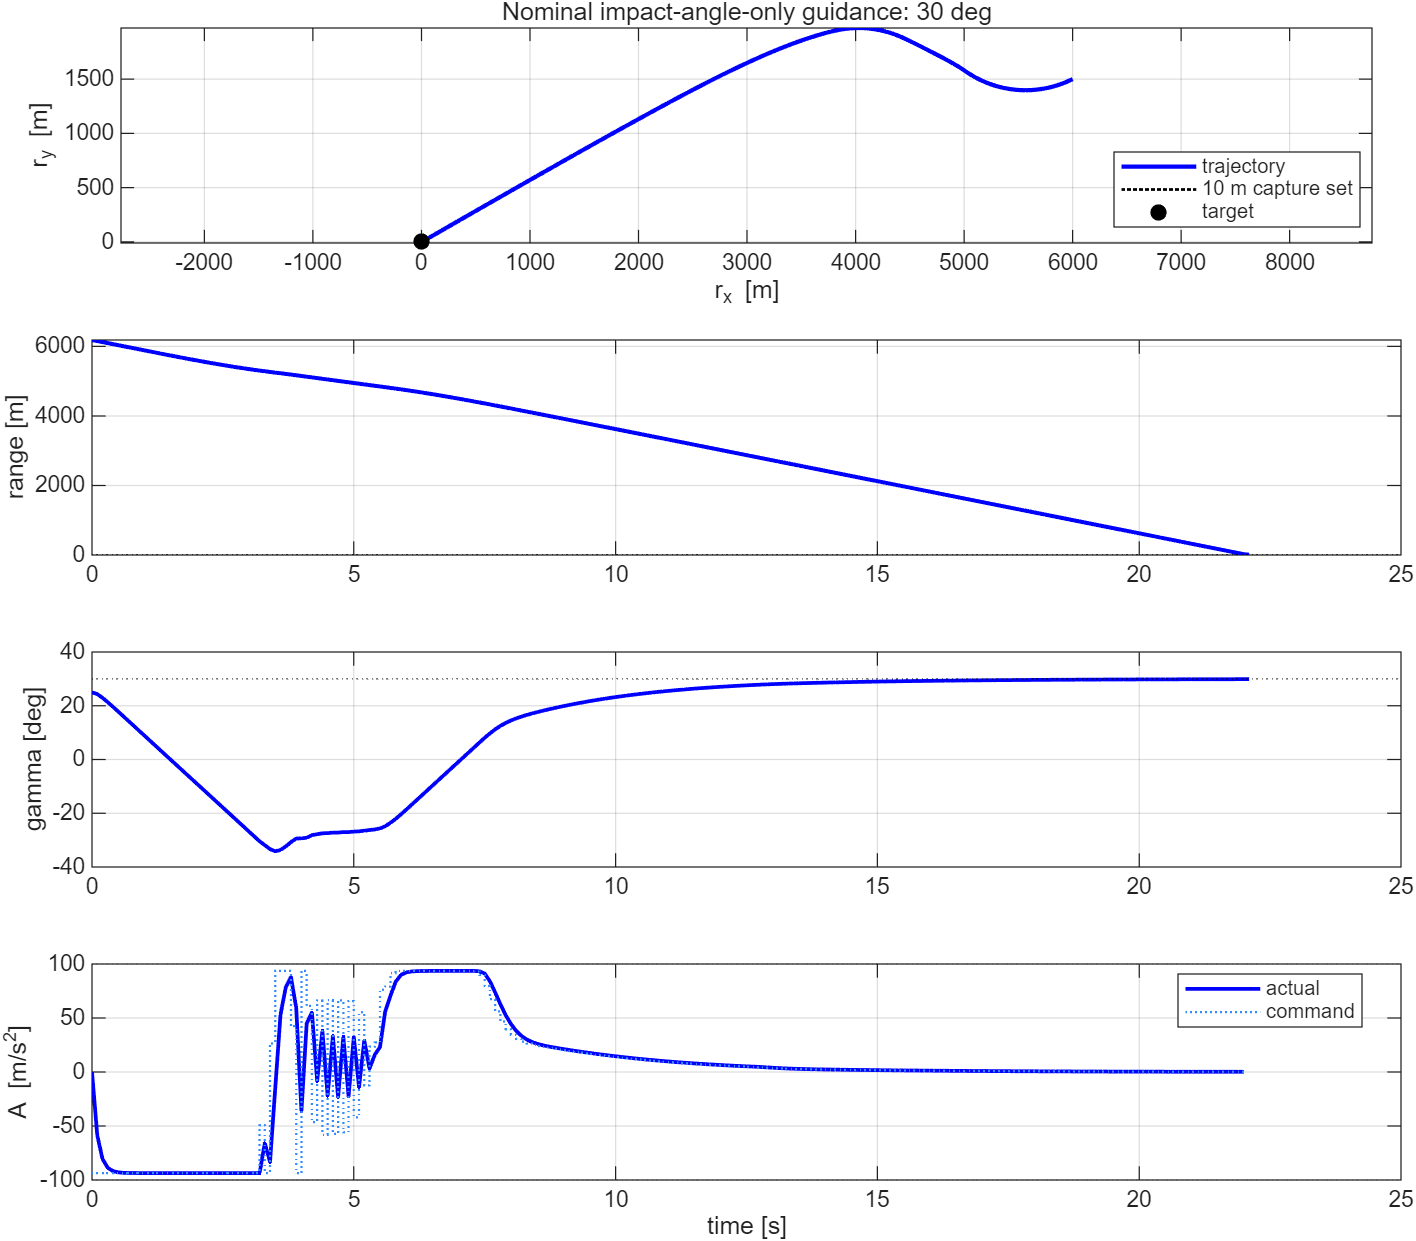
\includegraphics[width=3.35in]{KDPC_RSRFG-main/StationaryTargetKoopman/results/closed_loop_angle_30_nominal.png}}
\hfil
\subfloat[45$^\circ$ impact-angle command.]{
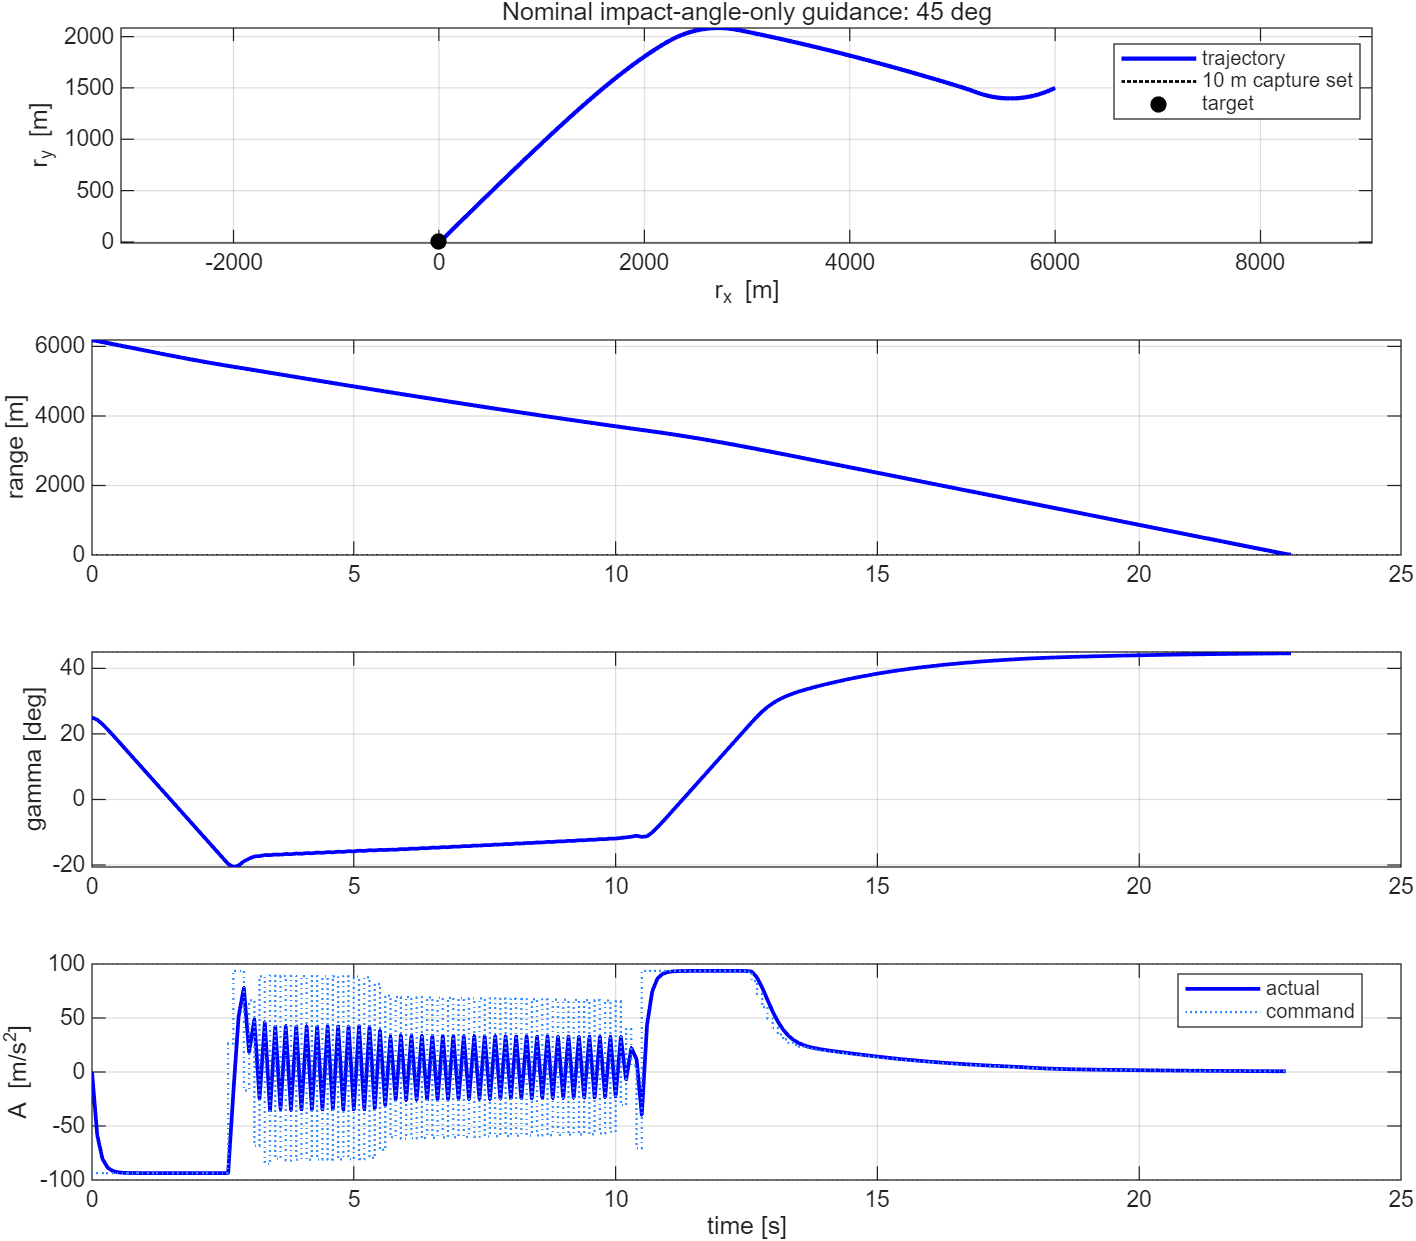
\includegraphics[width=3.35in]{KDPC_RSRFG-main/StationaryTargetKoopman/results/closed_loop_angle_45_nominal.png}}
\caption{Nominal flight simulations for the 30$^\circ$ and 45$^\circ$ impact-angle-only cases. Each plot shows the trajectory, range, heading, and first-order-autopilot lateral acceleration.}
\label{fig:angle_only_nominal}
\end{figure*}

\section{Discussion}
The results support three conclusions. First, the use of $[\tau/t_f,y/R_s,\theta]^T$ is not merely a numerical convenience. It changes the terminal guidance problem into a form in which the desired impact condition is an origin of the terminal error state. This makes terminal-set, recursive-feasibility, and ISS statements meaningful. Second, the exact continuous-time bilinear Koopman derivation for the ideal core explains why a bilinear predictor is structurally better matched to the guidance dynamics than a purely linear input predictor. The validation results confirm this point over the 35-step prediction horizon even when the learned predictor includes the first-order autopilot state. Third, residual-tube tightening gives a concrete way to account for finite-dimensional prediction error when terminal constraints are enforced through a learned predictor.

From a theoretical point of view, the manuscript is complete in three parts: the controlled Koopman generator is well defined under Assumption 1, the Cartesian lifted model gives an exact finite-dimensional continuous-time bilinear representation for the ideal guidance core, and the time-to-go lateral-error state converts the scheduled terminal condition into an origin constraint. The bilinear EDMD predictor, sequential convex quadratic program, first-order-autopilot augmentation, and validation-data tube then provide a complete implementable nominal guidance algorithm. The remaining theoretical gap is narrower but important: the current code uses a tightened polyhedral terminal approximation rather than a computed invariant Lyapunov terminal set. Therefore, the recursive-feasibility and ISS statements should be read as conditional design statements based on \eqref{eq:terminal_set} and \eqref{eq:iss_condition}, not yet as a fully closed formal proof for every initial condition in a specified domain.

The current study also has clear boundaries. The model is a nominal stationary-target model with first-order autopilot dynamics; it does not yet include target maneuvers, aerodynamic drag, higher-order autopilot loops, or field-of-view constraints. The terminal screening cases show that the 10 m capture set can be missed even when the impact-angle error is small, especially when the requested impact time or impact angle moves outside the current reachable envelope. Thus, future work should compute $\mathcal X_f(\tau)$ explicitly, enlarge the training and prediction domains, and introduce reachability-based terminal-time selection before moving to disturbance compensation or moving-target extensions.

\section{Conclusion}
This paper presented a tube-tightened bilinear Koopman-MPC framework for nominal planar guidance with simultaneous impact-time and impact-angle constraints. The theory separates an exact continuous-time bilinear Koopman representation of the ideal guidance core from the finite-dimensional data-driven predictor used for online optimization. A time-to-go lateral-error state makes the prescribed terminal condition a true origin, which provides a suitable basis for terminal-set and ISS-style analysis. The implementation combines bilinear EDMD, first-order autopilot augmentation, sequential convex quadratic programming, terminal residual-tube tightening, interpolation of the lifted initial state, and an input-difference penalty. Simulations with a 10 m capture radius show successful nominal fixed-time interception at 21.70 s and 21.75 s for $\gamma_f=-2^\circ$, with the baseline case achieving a 5.978 m miss distance and a $0.647^\circ$ impact-angle error. Additional screening cases reveal the reachable envelope of the current design. Future work will replace the current terminal polytope approximation with a rigorously computed $\mathcal X_f(\tau)$ and extend the formulation to moving targets, aerodynamic effects, and higher-order autopilot dynamics.

\balance
\begin{thebibliography}{99}

\bibitem{koopman1931}
B. O. Koopman, ``Hamiltonian systems and transformation in Hilbert space,'' \emph{Proceedings of the National Academy of Sciences}, vol. 17, no. 5, pp. 315--318, 1931.

\bibitem{williams2015edmd}
M. O. Williams, I. G. Kevrekidis, and C. W. Rowley, ``A data-driven approximation of the Koopman operator: Extending dynamic mode decomposition,'' \emph{Journal of Nonlinear Science}, vol. 25, no. 6, pp. 1307--1346, 2015.

\bibitem{korda2018mpc}
M. Korda and I. Mezic, ``Linear predictors for nonlinear dynamical systems: Koopman operator meets model predictive control,'' \emph{Automatica}, vol. 93, pp. 149--160, 2018.

\bibitem{bevanda2021kodm}
P. Bevanda, S. Sosnowski, and S. Hirche, ``Koopman operator dynamical models: Learning, analysis and control,'' \emph{Annual Reviews in Control}, vol. 52, pp. 197--212, 2021.

\bibitem{dejong2024kdpc}
T. de Jong, V. Breschi, M. Schoukens, and M. Lazar, ``Koopman data-driven predictive control with robust stability and recursive feasibility guarantees,'' in \emph{Proc. 63rd IEEE Conference on Decision and Control}, 2024, pp. 140--145.

\bibitem{zhou2024klmpc}
M. Zhou, M. Lu, G. Hu, Z. Guo, and J. Guo, ``Koopman operator-based integrated guidance and control for strap-down high-speed missiles,'' \emph{IEEE Transactions on Control Systems Technology}, vol. 32, no. 6, pp. 2436--2449, 2024.

\end{thebibliography}

\end{document}
